\section{Three-flavor \chpt\ to leading order}
\label{section: three-flavor chpt to leading order}

We will begin by considering the leading order Lagrangian, which chiral dimension $D=2$.
However, we will not include the $\text{QED}$ Lagrangian, as we will not consider electromagnetic interaction beyond leading order.
In this case, the dynamics of the photon will not contribute.
With this, the leading order Lagrangian is~\autocite{eckerRoleResonancesChiral1989,gasserChiralPerturbationTheory1984,gasserChiralPerturbationTheory1985,schererIntroductionChiralPerturbation2002}
%
\begin{equation}
    \label{leading order three-flavor Lagrangian}
    \Ell_2 
    = \frac{1}{4}f^2 \Tr{\nabla_\mu \Sigma \nabla^\mu \Sigma^\dagger}
    + \frac{1}{4}f^2 \Tr{\chi \Sigma^\dagger + \Sigma \chi^\dagger}
    + e^2 C \Tr{\Sigma Q_L \Sigma^\dagger Q_R}.
\end{equation}
%
We will work with three flavors, i.e. $N_f = 3$, so the mass matrix is now
%
\begin{equation}
    m = 
    \begin{pmatrix}
        m_u & 0 & 0 \\
        0 & m_d & 0 \\
        0 & 0 & m_s
    \end{pmatrix}.
\end{equation}
%
When we evaluate $s = m$ and $p = 0$, the scalar term then becomes
%
\begin{equation}
    \chi = 2B_0 m = 
    \begin{pmatrix}
        \bar m^2 - \Delta m^2 & 0 &0\\
        0& \bar m^2 + \Delta m^2 & 0 \\
        0&0&m_S^2
    \end{pmatrix},
\end{equation}
%
where we have defined
%
\begin{equation}
    \bar m^2 =  B_0(m_u + m_d),\quad 
    \Delta m^2 = B_0(m_d - m_u), \quad
    m_S^2 = 2B_0 m_s.
\end{equation}
%
The charge matrix is
%
\begin{equation}
    \label{three-flavor charge matrix}
    Q = \frac{1}{3}
    \begin{pmatrix}
        2 & 0 & 0\\
        0 & -1 & 0\\
        0 & 0 & -1
    \end{pmatrix}
    = \frac{1}{2} \left( \lambda_3 + \frac{1}{\sqrt{3}} \lambda_8 \right).
\end{equation}
%
In the vacuum, when there are no external currents, we choose the standard, exponential parametrization of the Goldstone manifold,
%
\begin{equation}
    \Sigma(x) = \exp{i\frac{\varphi_a \lambda_a}{f}}.
\end{equation}
%
Here, $\lambda_\alpha$ are the Gell-Mann matrices, as shown in \autoref{section: algebra bases}, are generators of $\Lie{SU}{3}$, and $f$ is the bare pion decay constant.
There are eight Goldstone bosons, $\varphi_a$, which are real functions of space-time.
This parametrization ensures that $\varphi = 0$ corresponds to the vacuum.
Using the isospin transformation rule \autoref{sigma transform under H}, we can perform an infinitesimal transformation of the Goldstone fields,
%
\begin{equation}
    \Sigma \rightarrow U_V \Sigma U_V^\dagger
    \sim
    \left(1 + i \eta_a \frac{1}{2} \lambda_a\right)
    \left(1 + i \frac{1}{f} \varphi_b  \lambda_b\right)
    \left(1 - i \eta_c \frac{1}{2} \lambda_c\right)
    \sim
    1 + i\frac{\varphi_a}{f} \lambda_a + i \frac{\varphi_a}{f} \eta_b f_{abc} \lambda_c,
\end{equation}
%
or
%
\begin{equation}
    \varphi_a \rightarrow [\delta_{ab} + i\eta_\alpha (-if_{\alpha ab})] \varphi_b.
\end{equation}
%
That is, $\varphi_a$ transforms under the adjoint representation of $\lie{su}{3}$, which is made up of elements of the form $\eta_\alpha (-i f_{\alpha ab})$.
The $\lie{su}{3}$ Lie algebra has three independent $\lie{su}{2}$ sub-algebras.
We introduce the matrices
%
\begin{equation}
    \lambda_Q = \lambda_3 + \frac{1}{\sqrt{3}}\lambda_8, \quad
    \lambda_K = -\lambda_3 + \frac{1}{\sqrt{3}}\lambda_8,
\end{equation}
%
From the structure constants, \autoref{structure constants su(3)}, we can conclude that they commute, i.e., $[\lambda_Q, \lambda_K] = 0$.
Furthermore, we find the commutation relations
%
\begin{equation}
    [\lambda_i, \lambda_j] = 2i \epsilon_{ijk} \lambda_k,\quad
    ijk \in \{1, 2, 3\}, \, \{4, 5, Q\}, \, \text{or} \, \{6, 7, K\}.
\end{equation}
%
We here define the Levi-Civita symbol by $\epsilon_{123} = \epsilon_{34Q} =\epsilon_{67K} = 1$.
This is the defining commutation relation of $\lie{su}{2}$.
The first subalgebra, spanned by $\{ \lambda_1, \lambda_2, \lambda_3 \}$, corresponds to isospin transformations, which are rotations of the up and down quark into each other.
Consider the transformation where $\eta_3 \neq 0$, while $\eta_\alpha = 0$ for $\alpha \neq 3$.
Acting on the quarks, this transformation is generated by $\lambda_3$, while in the adjoint representation the generator is $f_{3ab}$.
Under this transformation,  $\varphi_3\lambda_3$ is invariant.
We can see this from the fact that the structure constants $f_{abc}$ is totally antisymmetric, and thus $f_{33b} = 0$.
This means that $\varphi_3$ has the quantum number $I_3 = 0$.
$\varphi_1\lambda_1$ and $\varphi_2\lambda_2$ do not have definite values of the third component of isospin as they are not eigenvectors of $f_{3ab}$, but they do have definite values for the first and second component.
The linear combinations $\pi^\pm \, (\lambda_1 \mp \lambda_2)$, on the other hand, do.
This shows the relationship between our fields $\varphi_a$, and the observed, charged pions $\pi^+$ and $\pi^-$, as they have definite values for $I_3$.\footnote{
    Authors differ if they define $\sqrt 2 \pi^\pm = \varphi_1 \pm i \varphi_2$, or with opposite signs, $\sqrt 2 \pi^\pm = \varphi_1 \mp i \varphi_2$.  We choose the latter, so that $\pi_+ \ket{0}$ is the state with the quantum numbers of the positive pion.
    }
The full relationship between the $\varphi_a$-fields  and the observed pseudoscalar mesons is~\autocite{schererIntroductionChiralPerturbation2002}
%
\begin{equation}
    \varphi_a \lambda_a
    =
    \begin{pmatrix}
        \varphi_3 + \frac{1}{\sqrt{3}} \varphi_8 & \varphi_1 - i \varphi_2 & \varphi_4 - i \varphi_5 \\
        \varphi_1 + i \varphi_2 & - \varphi_3 + \frac{1}{\sqrt{3}} \varphi_8 & \varphi_6 - i \varphi_7  \\
        \varphi_4 + i \varphi_5 & \varphi_6 + i \varphi_7  & - \frac{2}{\sqrt{3}} \varphi_8
    \end{pmatrix}
    =
    \begin{pmatrix}
        \pi^0 + \frac{1}{\sqrt{3}}\eta & \sqrt{2}\pi^+ & \sqrt{2}K^+ \\
        \sqrt{2}\pi^- & -\pi^0 + \frac{1}{\sqrt{3}}\eta & \sqrt{2}K^0 \\
        \sqrt{2}K^- & \sqrt{2}\bar K^0  & - \frac{2}{\sqrt 3} \eta
    \end{pmatrix}.
\end{equation}




\subsection{Ground state}

When we take into account chemical potentials, we need to pick a new parametrization.
We will start the analysis by assuming $e = 0$ and then reintroduce electromagnetic interactions later.
The covariant derivative is then
%
\begin{equation}
    \nabla_\mu \Sigma = \partial_\mu \Sigma - i [v_\mu, \Sigma], \quad 
    v_\mu = \mu \delta^0_\mu.
\end{equation}  
%
The chemical potential matrix $\mu$ has three independent degrees of freedom, one for each quark, and is
%
\begin{equation}
    \mu = 
    \begin{pmatrix}
        \mu_u & 0 & 0 \\
        0 & \mu_d & 0 \\
        0 & 0 & \mu_s
    \end{pmatrix}
    = 
    \begin{pmatrix}
        \frac{1}{3}\mu_B + \frac{1}{2}\mu_I & 0 & 0 \\
        0 & \frac{1}{3}\mu_B - \frac{1}{2}\mu_I & 0 \\
        0 & 0 & \frac{1}{3}\mu_B - \mu_S
    \end{pmatrix}
    = \frac{1}{3}(\mu_B - \mu_S) \one 
    + \frac{1}{2} \mu_I \lambda_3
    + \frac{1}{\sqrt{3}}\mu_S\lambda_8,
\end{equation}
%
where we have defined $\mu_B = \frac{3}{2}(\mu_u + \mu_d)$, $\mu_I = \mu_u - \mu_d $ and $\mu_S = \frac{1}{2}(\mu_u + \mu_d)-\mu_s$.
Here, $\mu_u$, $\mu_d$, and $\mu_s$ are the up, down, and strange quark chemical potentials, while $\mu_B$, $\mu_I$, and $\mu_S$ are the baryon number, isospin, and strangeness chemical potentials.
$\Sigma$ transforms as $\Sigma \rightarrow \Sigma$ under $U(1)_V$, the symmetry corresponding to the baryon number; it is a baryon number singlet.
This reflects the fact that the baryon number of mesons, and thus the $\varphi_a$'s, is zero.
Therefore, the chemical potential corresponding to the baryon number, $\mu_B$, should not affect the final result.
We can also see this because $\mu_B$ only appears with the identity matrix $\one$ in $\mu$.
Any dependence on $\mu_B$ in $\nabla_\mu \Sigma$ will vanish as $\one$ commutes with everything.

We will assume the ground state is a spatially independent configuration, $\varphi_a^0 =\const$
This configuration must then minimize the free energy, too leading order, is equivalent to minimizing the static Hamiltonian, i.e., $\He^{(0)} = \He[\varphi^0]$.
To this end, we define
%
\begin{equation}
    \Sigma_\alpha 
    = \exp{i \alpha n_a \lambda_a},
    \quad \alpha = \frac{1}{f} \sqrt{\varphi_a^0 \varphi_a^0}, \quad n_a = \frac{\varphi_a^0}{\sqrt{\varphi_b^0 \varphi_b^0}}. 
\end{equation}
%
We show how to derive the correct parametrization of the ground state in the case of two flavors in \autoref{section: leading order}.
For $\mu_S = 0$, we expect to recover this result, in which $n_1^2 + n_2^2 =1$, and thus $n_a = 0$ for $a>2$.
Furthermore, we showed that we may choose $n_1 = 0$ without loss of generality, in which case the ground state becomes
%
\begin{equation}
    \Sigma_\alpha^{\pipm} = \exp{i \alpha \lambda_2} = (\one - \lambda^2_2) + \lambda_2^2 \cos\alpha + i \lambda_2\sin\alpha.
\end{equation}
%
The ground state is thus parameterized by $\alpha$ only.
As we will show in \autoref{chapter: thermodynamics}, when the isospin chemical potential exedes a critical value, $\mu_I \geq \mu_I^c$, the system undergoes a phase transition from the vacuum phase to a phase in which $\alpha \neq 0$, and the charged pions form a condensate.
It is only when we reach this phase that the equation of state is non-trivial at $T=0$, which makes it possible for pion stars to form.

If we define $\mu_\Kpm = \mu_S + \frac{1}{2}\mu_I$ and $\mu_\Ko = \mu_S - \frac{1}{2}\mu_I$, then we can write the terms of the QCD Lagrangian made up of $\mu_I$ and $\mu_S$ and their corresponding currents densities as
%
\begin{equation}
    \bar q \gamma^0\left(\frac{1}{2}\mu_I \lambda_3 + \frac{1}{\sqrt 3}\mu_S \lambda_8 \right) q
    = 
    \bar q\gamma^0 \left( \frac{1}{2}\mu_\Kpm \lambda_Q + \frac{1}{2} \mu_\Ko \lambda_K\right) q.
\end{equation}
%
Analogously to how a higher $\mu_I$ leads to a condensate in the first $\lie{su}{2}$ subalgebra, we can expect these chemical potentials to lead to different condensates in their respective subalgebras.
If we assume $\mu_\Ko = 0$, we would expect the new ground state to take the form
%
\begin{align}
    \Sigma_\alpha^{\Kpm} = \exp{i \alpha \lambda_5} = (\one - \lambda^2_5) + \lambda_5^2 \cos\alpha + i \lambda_5\sin\alpha.
\end{align}
%
This analysis extends to all four quadrants of the $\mu_I-\mu_S$ plane.
If we set $\mu_\Kpm = 0$, we would expect a ground state of the form $e^{i\alpha\lambda_7}$.
In \autocite{kogutQCDSmallNonzero2001}, \citeauthor{kogutQCDSmallNonzero2001} show that this analysis is right, and that these states are local minima of the static Lagrangian.
However, the domains of the different condensates overlap, so there is a phase transition between the condensates.
We will study the different condensates and the transition between them in \autoref{chapter: thermodynamics}.



\subsection{The pion-condensed phase}
\label{subsection: pion-condensed phase}

The new ground state $\Sigma_\alpha$ is a rotation of the vacuum state $\Sigma_0 = \one$ by $U_A = A_\alpha^i$.
To parameterize excitations from this new field, we must then rotate the excitations $U(x)$ accordingly.
The procedure is shown in detail for the two-flavor case in \autoref{section: two-flavor chpt to leading order}.
This new parametrization is
%
\begin{equation}
    \Sigma(x) = A^i_\alpha U(x) \Sigma_0 U(x) A^i_\alpha, \quad
    U(x) = \exp{i \frac{\varphi_a \lambda_a}{2 f}}, \quad
    A_\alpha^i = \exp{i \frac{\alpha \lambda_i}{2}},
\end{equation}
%
where $i = 2, 5, 7$ depending on which phase we are in.
We begin the analysis of the pion-condensed phase, so $i = 2$, and assume $\mu_I > 0$ and $e = 0$.
Inserting this into \autoref{leading order three-flavor Lagrangian}, and expanding up to and including $\Oh\left((\pi/f)^2\right)$, we get
%
\begin{align}
    \label{static three-flavor Lagrangian}
    \Ell_2^{(0)} 
    &=
    \frac{1}{2} f^2
    \left(
        \mu_I^2 \sin^2\alpha
        + 2\bar m^2 \cos\alpha
        + m_S^2
    \right), \\
    \label{linear three-flavor Lagrangian}
    \Ell_2^{(1)}
    &=
    -f \mu_I \partial_0 \varphi_1 \sin\alpha
    + f \sin\alpha
    \left(
        \mu_I^2\cos\alpha - \bar m^2
    \right)\varphi_2, \\
    \label{quadratic three-flavor Lagrangian}
    \Ell_2^{(2)} 
    &= 
    \frac{1}{2}\partial_\mu \varphi_a \partial^\mu \varphi_a
    + \frac{1}{2} m_{ab} \varphi_a\partial_0\varphi_b
    - \frac{1}{2} m_a^2 \varphi_a^2
    - \frac{1}{\sqrt{3}} \Delta m^2 \varphi_3 \varphi_8.
\end{align}
%
Here, we have introduced a number of mass parameters, which will in general be functions of $\alpha$ and the chemical potentials.
The diagonal mass terms are
%
\begingroup
\allowdisplaybreaks
\begin{align}
    \label{m1}
    m_1^2 &=  \bar m^2\cos\alpha - \mu_I^2 \cos^2\alpha,\\
    m_2^2 &= \bar m^2\cos\alpha - \mu_I^2 \cos2\alpha, \\
    m_3^2 &= \bar m^2\cos\alpha + \mu_I^2 \sin^2\alpha, \\
    m_4^2 &= m_5^2 = m_-^2 - m_{\mu+}^2, \\
    m_6^2 &= m_7^2 = m_+^2 - m^2_{\mu-}, \\
    \label{m8}
    m_8^2 &= \frac{1}{3} (\bar m^2 \cos\alpha + 2 m_S^2),
\end{align}
\endgroup
%
where
%
\begin{equation}
    \label{mass terms in pion condensate}
    m_\pm^2 = \frac{1}{2} (\bar m^2 \cos\alpha \pm \Delta m^2 + m_S^2),
    \quad
    m^2_{\mu\pm } = \left(\pm \mu_S + \frac{1}{2}\mu_I\cos\alpha \right)^2 
    - \frac{1}{4}\mu_I^2 \sin^2\alpha,
\end{equation}
%%
and the off-diagonal terms are
%%
\begin{align}
    \label{m12}
    m_{12} & = 2 \mu_I\cos\alpha,\\
    m_{45} & = 2 \left( \mu_S + \frac{1}{2} \mu_I  \cos\alpha\right), \\
    \label{m76}
    m_{67} & =  2 \left( - \mu_S + \frac{1}{2} \mu_I  \cos\alpha\right).
\end{align}
%
Here, $m_{ab} = -m_{ba}$, and terms not defined above are zero.
These terms mean that the basis $\varphi_a$ does not correspond to mass eigenstates.
This is to be expected, as they are not eigenstates of isospin nor strangeness.

At $\mu_S = \mu_I = 0$ and $\alpha = 0$, we obtain the well-known, tree-level masses of the pseudoscalar mesons~\autocite{eckerChiralPerturbationTheory1995},
%
\begin{align}
    \label{leading order pion mass mu=0}
    m_{\pi,0}^2 &
    = \bar m^2 
    = B_0(m_u + m_d)\\
    \label{leading order charged kaon mass mu=0}
    m_{\Kpm, 0}^2 
    & = \frac{1}{2} (\bar m^2 - \Delta m^2 + m_S^2) 
    = B_0(m_u + m_s), \\
    \label{leading order neutral kaon mass mu=0}
    m_{\Ko, 0}^2
    & = \frac{1}{2} (\bar m^2 + \Delta m^2 + m_S^2) 
    = B_0(m_d + m_s), \\
    \label{leading order eta mass mu=0}
    m_{\eta, 0}^2
    &= \frac{1}{3}(\bar m^2  + 2m_S^2) 
    = \frac{1}{3}B_0(m_u + m_d + 4m_s).
\end{align}
%
To leading order, these are the physical masses of the pions, charged kaons, neutral kaons, and the $\eta$-particle.
The values used in this thesis are given in \autoref{section: units}.
Similarly, the $f$-constant is, to leading order, given by $f = f_\pi$.

To find the physical masses in the pion-condensed phase, we must analyze the propagator and the spectrum of the theory.
We follow~\autocite{adhikariTwoflavorChiralPerturbation2019,adhikariQuarkPionAxial2021}.
The spectrum is given by the zero of the inverse propagator, which has a block diagonal form.
In momentum space, it reads
%
\begin{align}
    \label{inverse propagator}
    D_{ab}^{-1} 
    &= \fdv{S}{\varphi_a,\varphi_b}
    =
    (p^2 - m_a^2)\delta_{ab} - i p_0 m_{ab}
    =
    \begin{pmatrix}
        D_{12}^{-1}   &0&0&0&0\\
        0& p^2 - m_3^2  &0&0&0\\
        0&0& D_{45}^{-1}  &0&0\\
        0&0&0& D_{67}^{-1}  &0\\
        0&0&0&0&p^2 - m_3^2 
    \end{pmatrix}
\end{align}
%
where
%
\begin{align}
    D_{12}^{-1}
    = 
    \begin{pmatrix}
        p^2 - m_1^2 & -ip_0 m_{12} \\
        ip_0 m_{12} & p^2 - m_1^2           
    \end{pmatrix}, \quad
    D_{45}^{-1}
    = 
    \begin{pmatrix}
        p^2 - m_4^2 & -ip_0 m_{45} \\
        ip_0 m_{45} & p^2 - m_5^2           
    \end{pmatrix}, \quad
    D_{67}^{-1}
    = 
    \begin{pmatrix}
        p^2 - m_6^2 & -ip_0 m_{ 67} \\
        ip_0 m_{67} & p^2 - m_7^2           
    \end{pmatrix}.
\end{align}
%
We have chosen to neglect the $\pi^0 - \eta$-mixing terms $D_{83}^{-1} = D_{38}^{-1} = - \Delta m^2 / \sqrt{3}$.
We will, however, keep $\Delta m \neq 0$ in the other mass contribution.
The spectrum of the theory is given by the zeros of the determinant of the propagator,
\begin{align}
    \nonumber
    \det\left(D^{-1}\right)
    =&\,
    (p^2 - m_3^2)(p^2 - m_8^2)
    \left[ (p^2 - m_1^2)(p^2 - m_2^2) - p_0^2m_{12}^2  \right]\\
    &\times
    \left[ (p^2 - m_4^2)(p^2 - m_5^2) -  p_0^2m_{45}^2  \right]
    \left[ (p^2 - m_6^2)(p^2 - m_7^2) -  p_0^2m_{67}^2  \right]
    = 0.
\end{align}
%
Solving $\det(D^{-1}) = 0$ for $p_0^2$ gives eight roots $E_i^2$, one for each particle.
Writing the four-momentum as $p^\mu = (p_0, \vv p)$, these zeros are
%
\begingroup
\allowdisplaybreaks
\begin{align}
    \label{E1}
    E_{\pi^0}^2 &= |\vv p |^2 + m_3^2, \\
    \label{E2}
    E_\eta^2 &= |\vv p |^2 + m_8^2, \\
    E_\pipm^2
    & = |\vv p|^2 +
    \frac{1}{2}
    \left(
        m_1^2 + m_2^2 + m_{12}^2 
    \right)
    \mp
    \frac{1}{2}
    \sqrt{
        4|\vv p|^2m_{12}^2 
        +
        \left(
            m_1^2 + m_2^2 + m_{12}^2
        \right)^2
        - 4 m_1^2 m_2^2
    }, \\
    \label{E3}
    E_\Kpm^2
    & = |\vv p|^2 + m_4^2 + \frac{1}{2} m_{45}^2 
    \mp
    \frac{1}{2} m_{45} \sqrt{4|\vv p|^2 + 4 m_4^2 + m_{45}^2},\\
    \label{E4}
    E_\Ko^2
    &= |\vv p|^2 + m_6^2 + \frac{1}{2} m_{67}^2 
    \pm
    \frac{1}{2} m_{67} \sqrt{4|\vv p|^2 + 4 m_6^2 + m_{67}^2}.
\end{align}
\endgroup
%
The masses of the particles are given by the energy at $\vv p = 0$.
For $\alpha = 0$, which we will later show is valid for low $\mu$'s, we get a Zeeman-like splitting of the energies of the pions,
%
\begin{equation}
    E_0 =\sqrt{|\vv p|^2 + \bar m^2}, \quad
    E_\pipm = \sqrt{|\vv p|^2 + \bar m^2} \mp \mu_I.
\end{equation}
%
The kaons have a similar splitting, only due to the kaon chemical potentials $\mu_\Kpm$ and $\mu_\Ko$ instead.
The masses of the various mesons are shown in \autoref{fig: leading order masses mesons}.
These results use the relationship between $\mu_I$ and $\alpha$, which we derive in the next chapter.
In the lower plot, we see the Zeeman splitting of the pion masses, which persists until the mass of the positive pion vanishes.
As we explore further in the next chapter, this happens as the exact isospin symmetry $\Lie{U}{1}_{I_3} \subset \Lie{SU}{3}_V $ is broken spontaneously by the pion condensate, and $\pi^+$ is the corresponding Goldstone boson.
On the top, we see that the kaons also get this Zeeman splitting in the vacuum phase.
%
\begin{figure}
    \centering
    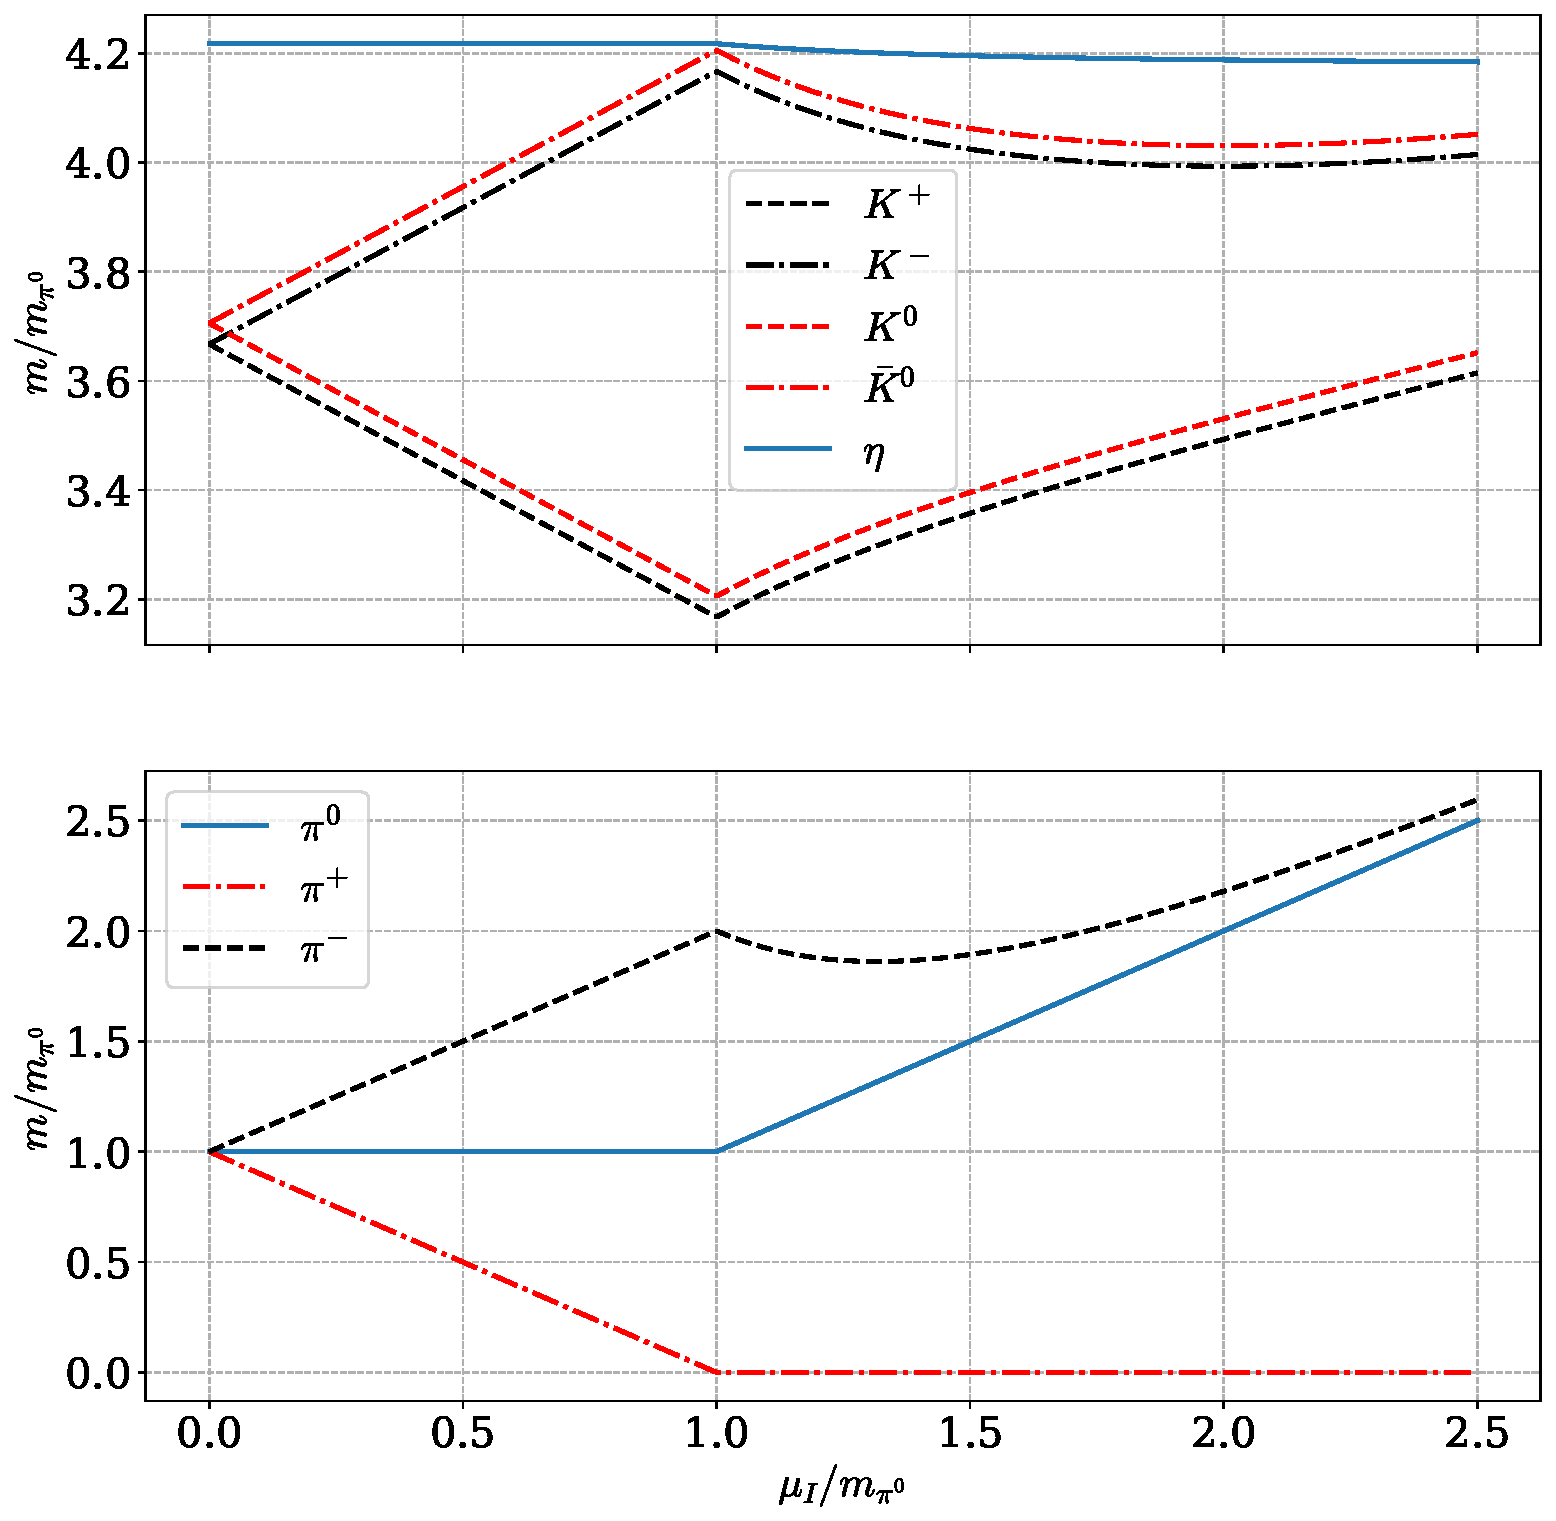
\includegraphics[width=0.8\textwidth]{../scripts/figurer/masses_mesons.pdf}
    \caption{
        The leading order masses of the pseudoscalar mesons, as functions of the isospin chemical potential.
        Both the masses and chemical potential are normalized to the pion mass.
        These results are at $\mu_S = 0$.
        The difference between the kaons at $\mu_I = 0$ is a result of the fact that $\Delta m \neq 0$.
        }
    \label{fig: leading order masses mesons}
\end{figure}
%

If we adjust the strangeness chemical potential instead, while the isospin chemical potential remains constant, then the kaons will get a similar splitting, as shown in \autoref{fig: leading order masses kaos afo strangeness}, while the pions are unaffected.
For $\mu_I > 0$, the mass of the positive kaon will reach zero first, at the point of transition into the charged kaon condensate.
At this point, the results obtained in this section will become invalid, as $\Sigma = \exp{i \alpha \lambda_2}$ no longer is the ground state.


\begin{figure}
    \centering
    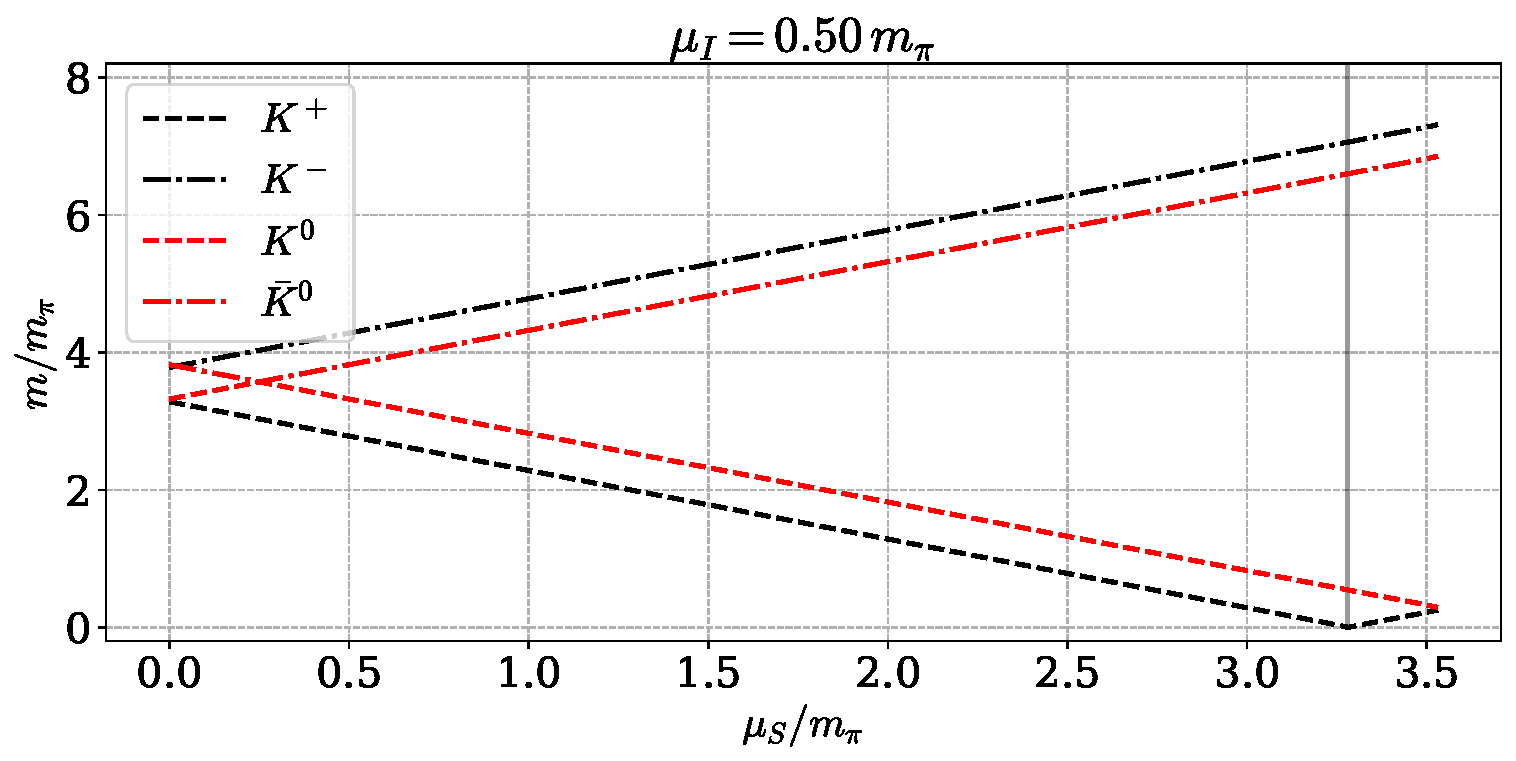
\includegraphics[width=0.8\textwidth]{../scripts/figurer/masses_kaons2.pdf}
    \caption{
        The kaon masses as a function of $\mu_S$, both in units of $m_\pi$, evaluated at $\mu_I = 0.5 \, m_\pi$.
        These results are only valid to the left of the gray line at $\mu_S\approx 3.3 \, m_\pi$, where $m_{K^+}$ reaches zero.
    }
    \label{fig: leading order masses kaos afo strangeness}
\end{figure}





\subsection{The kaon condensed phase}

In the $K^\pm$-condensate, we get
%
\begin{align}
    \label{static three-flavor Lagrangian kaon condensate}
    \Ell^{(0)}_2 
    & =
    \frac{1}{2}f^2 
    \left(
        \mu_\Kpm^2 \sin^2\alpha
        + 2m^2_{\Kpm, 0} \cos\alpha
        + \bar m^2 +\Delta m^2
    \right), \\
    \label{linear three-flavor Lagrangian kaon condensate}
    \Ell_2^{(1)}
    & 
    =
    - \frac{1}{2}f\mu_\Kpm\partial_0\varphi_4 \, \sin\alpha 
    + f\sin\alpha
    \left(
        \mu_\Kpm^2 \cos\alpha
        -m_{\Kpm,0}^2
    \right)\varphi_5\\
    \label{quadratic three-flavor Lagrangian kaon condensate}
    \Ell_2^{(1)}
    & =
    \frac{1}{2} \partial_\mu \varphi_a \partial^\mu \varphi_a
    + \frac{1}{2}m'_{ab} \varphi_a\partial_0\varphi_a
    - \frac{1}{2}m'^2_{a} \varphi_a^2
    - \frac{1}{2}\Delta_{\eta\pi} \varphi_3\varphi_8
\end{align}
%
where
\todo[]{Sjekk disse}
%
\begingroup
\allowdisplaybreaks
\begin{align}
    {m'}_{12} &= \frac{1}{2}(\cos\alpha + 3)\mu_I + (\cos\alpha - 1)\mu_S \\
    {m'}_{45} &= 2\mu_\Kpm\cos\alpha \\
    {m'}_{76} &= \frac{1}{2}(3-\cos\alpha) \mu_I - (1 + \cos\alpha)\mu_S, \\
    {m'}_1^2 & = m_2^2 = {m'}_-^2 + {m'}_{\mu-}^2,\\
    {m'}_3^2 
    & = 
    \frac{1}{4}
    \left(
        \mu_\Kpm^2 \sin^2\alpha
        + 2 m_{\Kpm, 0}^2\cos\alpha
        + 3\bar m^2
        + \Delta m^2
        - m_S^2
    \right),\\
    {m'}_4^2 & = m_{\Kpm,0}^2\cos\alpha -\mu_\Kpm \cos^2\alpha, \\
    {m'}_5^2 & = m_{\Kpm,0}^2\cos\alpha -\mu_\Kpm \cos 2\alpha, \\
    {m'}_6^2 & = m_7^2 = {m'}_+^2 + {m'}_{\mu+}^2,
\end{align}
\begin{align}
    {m'}_8^2
    & =
    \frac{1}{12}
    \left[
        \frac{9}{4}\mu_{\Kpm,0}^2\sin^2\alpha
        + \bar m^2(5\cos\alpha-1) 
        + 5\Delta m^2(\cos\alpha-1)
        + m_S^2(5\cos\alpha+3))
    \right], \\
    \Delta_{\eta\pi}
    & =
    \frac{\sqrt{3}}{2}
    \left[
        \mu_\Kpm^2\sin^2\alpha
        + \frac{1}{3}\bar m^2(\cos\alpha - 1)
        + \frac{1}{3}\Delta m^2(\cos\alpha + 3)
        + \frac{1}{3}m^2_S(\cos\alpha - 1)
    \right],
\end{align}
\endgroup
%
and
%
\begingroup
\allowdisplaybreaks
\begin{align}
    {m'}_\pm^2
    & =
    \frac{1}{4}\bar m^2 (\cos\alpha \mp 1 + 2)
    + \frac{1}{4} \Delta m^2 (\cos\alpha \mp 1-2)
    +\frac{1}{4} m_S^2 (\cos\alpha \pm 1), \\
    {m'}_{\mu\pm}^2
    & =
    \frac{1}{2}(\sin^2\alpha  \pm 3\cos\alpha - 5)\mu_I^2
    +(\sin^2\alpha\pm\cos\alpha + 1)\mu_I\mu_s
    +(\sin^2\alpha\mp\cos\alpha - 1)\mu_s^2.
\end{align}
\endgroup
%
We see that both the Lagrangian and the masses have a similar structure to the pion condensate, only with $\varphi_4$ and $\varphi_5$ taking the roles of $\varphi_1$ and $\varphi_2$, and $\mu_\Kpm$ and $m_\Kpm$ the roles of $\mu_I$ and $\bar m$.
The phase with a $\Ko$-condensate, with the ground state $\Sigma = \exp{i \lambda_7 \alpha}$ has a very similar structure.
The static Lagrangian is
%
\begin{equation}
    \label{static Lagrangian neutral kaon}
    \Ell_2^{(0)} = \frac{1}{2}f^2 
    \left(
        \mu_\Ko^2 \sin^2\alpha
        + 2m_\Ko^2\cos\alpha + \bar m^2 - \Delta m^2
    \right).
\end{equation}
%


 
\subsection{Electromagnetic contributions}

We now reintroduce $e$.
First, we set $\mu_I = \mu_S = 0$, so we are in the vacuum phase, $\Sigma = U^2 = \exp{i \varphi_a \lambda_a/f}$, and the covariant derivative is
%
\begin{equation}
    \nabla_\mu \Sigma = \partial_\mu \Sigma - i e \mathcal A_\mu [Q, \Sigma],
\end{equation}
%
where $Q$ is the charge matrix \autoref{three-flavor charge matrix}.
Inserting this into the terms of the leading-order Lagrangian, \autoref{leading order three-flavor Lagrangian}, and expanding to and including $\Oh\left((\pi/f)^2\right)$ yields
%
\begin{align}
    \nonumber
    \Ell_2
    &= 
    \frac{1}{2} \partial_\mu \varphi_a \partial^\mu \varphi_a
    - \frac{1}{2}(m_{a}^2 + \Delta m_{\text{EM},a}^2)\varphi_a^2
    - \frac{\Delta m^2}{\sqrt 3} \varphi_3 \varphi_8
    + f^2 \left(\bar m^2 + \frac{1}{2} m_S^2 + \frac{2}{3}\frac{C e^2}{f^2}\right)\\
    &+ e \mathcal A^\mu 
    (
        \varphi_1 \partial_\mu \varphi_2
        - \varphi_2 \partial_\mu \varphi_1
        + \varphi_4 \partial_\mu \varphi_5
        - \varphi_5 \partial_\mu \varphi_4
    )
    + \frac{1}{2} e^2 \mathcal A^2 (\varphi_1^2 +\varphi_2^2 + \varphi_4^2 +\varphi_5^2).
\end{align}
%
Here, $m_{a}$ are the masses  we found in \autoref{leading order three-flavor Lagrangian}, at $\mu_I = \mu_S = \alpha = 0$, while $\Delta m_{\text{EM}, a}$ is the new electromagnetic contribution to the masses.
This only affects the charged pions $\pipm$, which are linear combinations $\varphi_1$ and $\varphi_2$, and the charged kaons, $\Kpm$, which are linear combinations of $\varphi_4$ and $\varphi_5$.
The contribution to mass from electromagnetic effects are, to leading order, the same for these particles,
%
\begin{equation}
    \Delta m_{\text{EM}, a}^2 = 2C \frac{e^2}{f^2} := \Delta m^2_\text{EM}, \quad a \in \{1, 2, 4, 5\}.
\end{equation}
%
This is known as Dashen's theorem~\autocite{dashenChiralMathrmSUEnsuremath1969}.
We can express $C$ in terms of the pion decay constant and the mass and decay constant of the $\rho$-meson.
This was first done in~\autocite{dasElectromagneticMassDifference1967}, using the then newly derived Weinberg sum rules relating the masses of heavier mesons~\autocite{weinbergPreciseRelationsSpectra1967}.
This yields
%
\begin{equation}
    \label{C from rho}
    C = \frac{3 m_\rho^2 f_\rho^2}{32 \pi^2} 
    \ln\left(  \frac{f_\rho^2}{f_\rho^2 - f_\pi^2}  \right),
\end{equation}
%
\citeauthor{urechVirtualPhotonsChiral1995}, using the values $f_\pi = 93.3\, \text{MeV}$, $f_\rho = 154 \text{MeV}$ and $m_\rho = 770\, \text{MeV}$, gets the numerical result $6.11\times 10^{-6} \, (\text{GeV})^4$~\autocite{urechVirtualPhotonsChiral1995}.
With the value $f_\pi = 92.1\,\text{MeV}$ as used in the rest of this text, we obtain $C = 5.90\times 10^{-6} \, (\text{GeV})^4$.
As $C$ is the sole source of difference in the masses of the neutral and charged pions to leading order, it can also be obtained directly from these masses.
Using the values listed in \autoref{section: units}, we find
%
\begin{equation}
    \label{C from pion masses}
    C= \frac{f^2}{2 e^2}(m_{\pi_\pm}^2 - m_{\pi}^2) = 5.824 \times 10^{-6} \, (\text{GeV})^4 ,
\end{equation}
%
or in the characteristic units of the system, $C = 0.3771 \, u_0$.
This corresponds to $\Delta m_\text{EM}^2 = 35.50 \, \text{MeV}$.
We see that the numerical differences between these results are small.
When choosing the numerical values to use, we must take care to use a consistent set of values.
Formulas such as \autoref{C from rho} mean that the decay constants and masses are over-constrained.
In this text, we use the masses and the decay constant listed in \autoref{section: units} and therefore choose the value in \autoref{C from pion masses} for $C$.

The contribution to the pion mass from electromagnetic interactions is
%
\begin{equation}
    m_\pipm - m_\pi = \left(\sqrt{1 + \Delta m_\text{EM}^2 / m_\pi^2} - 1\right) m_\pi
    = 3.401\times 10^{-2} \,m_\pi = 4.590\,\text{MeV}.
\end{equation}
%
Even though the contribution to the \emph{square} of the masses of the charged pion and kaons are the same, we see that the absolute difference between the neutral and charged pion depends on $\Delta m_\text{EM}/ m_\pi $.
We, therefore, expect the mass contribution from electromagnetic interactions to be lower for the heavier charged kaon.
From the values in \autoref{section: units}, however, we see that the mass difference between the charged and neutral pions masses are very close to that of the charged and neutral kaons.
This is because the difference in mass of the kaons is not only due to the electric charge at leading order, unlike the pions, but also due to $\Delta m$,
%
\begin{equation}
    m_\Ko^2 - m_\Kpm^2 = \Delta m^2 - \Delta m_\text{EM}^2.
\end{equation}
%
We notice that the two contributions work in opposite directions.
As we already have an independent way of determining $\Delta m_\text{EM}^2$, we can disentangle these contributions.
To leading order,
%
\begin{equation}
    \Delta m^2 
    = { m_\Ko^2 - (m_\Kpm^2 - \Delta m^2_\text{EM})}
    = 0.5320^2 \, m_\pi^2 = (71.80\, \text{MeV})^2.
\end{equation}
%
This is consistent with the fact that the down quark is around twice as heavy as the light quark~\autocite{particledatagroupReviewParticlePhysics2020}.
The electromagnetic contribution to the mass of the charged kaon is
%
\begin{equation}
    \left(1 - \sqrt{1 - \Delta m_\text{EM}^2/m_\Kpm^2} \right) m_\Kpm
    = 9.468 \times 10^{-3} \, m_\pi = 1.278 \, \text{MeV}.
\end{equation}
%
The difference due to $\Delta m$, on the other hand, is
%
\begin{equation}
    m_\Ko - \sqrt{m_\Kpm^2 - \Delta m_\text{EM}^2}
    = 3.858\,m_\pi = 5.208\, \text{MeV}.
\end{equation}

We analyze how electromagnetic interactions affect the condensed phases.
In the pion condensate, the covariant derivative is
%
\begin{equation}
    \nabla_\mu \Sigma = \partial_\mu \Sigma - i [v_\mu, \Sigma],
    \quad
    v_\mu = \mu \delta_\mu^0 + e \mathcal{A}_\mu Q.
\end{equation}
%
To zeroth order in $\pi/f$, the field parametrization is
%
\begin{equation}
    \Sigma = (\one - \lambda_2^2) + \lambda_2^2 \cos\alpha + i \lambda_2\sin\alpha.
\end{equation}
%
Inserting this in the leading-order Lagrangian \autoref{leading order three-flavor Lagrangian}, and setting $\mathcal A_\mu = 0$ gives us the static Lagrangian including electromagnetic effects,
%
\begin{equation}
    \label{static Lagrangian three-flavor EM}
    \Ell_2^{\text{EM}, (0)}
    =
    \frac{1}{2} f^2
    \left[
        (\mu_I^2 - \Delta m_\text{EM}^2)\sin^2\alpha + 2 \bar m^2\cos\alpha 
        + \frac{2}{3}\Delta m_\text{EM}^2 + m_S^2
    \right]
\end{equation}
%
Similarly, the static Lagrangian in the charged kaon condensate is
%
\begin{equation}
    \label{static Lagrangian three-flavor EM kaon}
    \Ell_2^{\text{EM}, (0)}
    =
    \frac{1}{2} f^2
    \left[
        (\mu_\Kpm^2 - \Delta m_\text{EM}^2) \sin^2\alpha + 2 m_{\Kpm,0}^2\cos\alpha 
        + \frac{2}{3}\Delta m_\text{EM}^2 + \bar m^2 + \Delta m^2
    \right]
\end{equation}
%
In the neutral kaon condensate, on the other hand, the static Lagrangian remains unchanged.

\begin{figure}
    \centering
    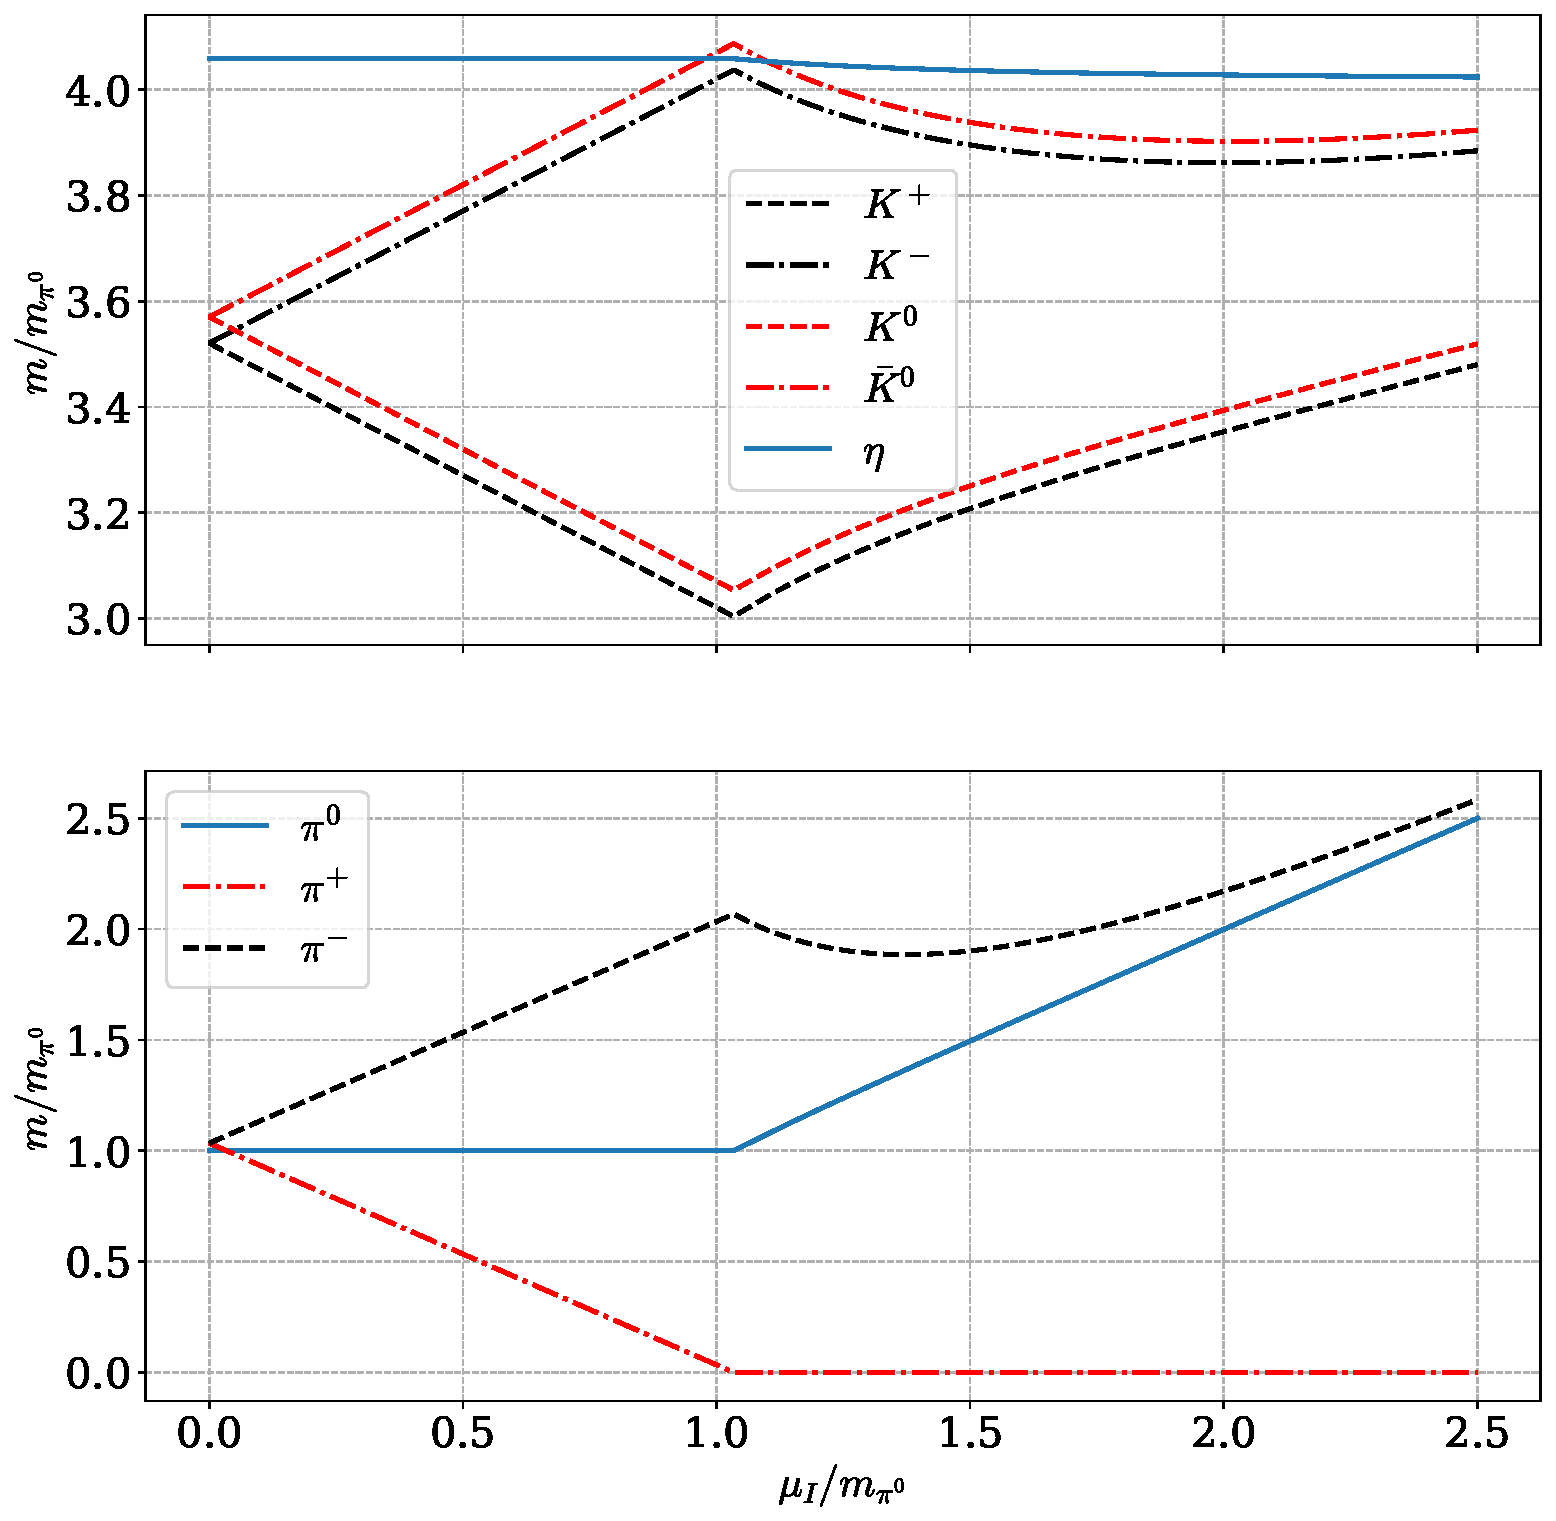
\includegraphics[width=0.8\textwidth]{../scripts/figurer/masses_mesons_EM.pdf}
    \caption{
        The leading order masses of the pseudoscalar mesons, as functions of the isospin chemical potential, including electromagnetic effects.
        Both the masses and chemical potential are normalized to the pion mass.
        These results are at $\mu_S = 0$.
        The difference between the kaons at $\mu_I = 0$ is a result of the fact that $\Delta m \neq 0$.
        }
    \label{fig: leading order masses mesons EM}
\end{figure}


In the pion condensate, the $\alpha$-dependent masses we found in \autoref{subsection: pion-condensed phase} are also affected by the inclusion of electromagnetic effects.
The diagonal mass terms are now 
%
\begingroup
\allowdisplaybreaks
\begin{align}
    m_1^2 &=  \bar m^2\cos\alpha - (\mu_I^2 - \Delta m_\text{EM}^2) \cos^2\alpha,\\
    m_2^2 &= \bar m^2\cos\alpha - (\mu_I^2  - \Delta m_\text{EM}^2)\cos2\alpha, \\
    m_3^2 &= \bar m^2\cos\alpha + (\mu_I^2  - \Delta m_\text{EM}^2)\sin^2\alpha, \\
    m_4^2 &= m_5^2 = m_-^2 - m_{\mu+}^2 + \frac{1}{2}\cos\alpha(\cos\alpha + 1) \Delta m_\text{EM}^2 , \\
    m_6^2 &= m_7^2 = m_+^2 - m^2_{\mu-} + \frac{1}{2}\cos\alpha(\cos\alpha - 1) \Delta m_\text{EM}^2, \\
    m_8^2 &= \frac{1}{3} (\bar m^2 \cos\alpha + 2 m_S^2),
\end{align}
\endgroup
%
where $m_\pm$ and $m_{\mu \pm}$ are defined as in \autoref{mass terms in pion condensate}.
These masses are illustrated in \autoref{fig: leading order masses mesons EM}.
